% fig_subset_sum_search: the three ideas of the subset-sum knapsack
% interdiction search (src/robust_ss.rs), on toy numbers.
% (a) Equal weights form classes; the leader only chooses how many copies of
%     each class survive (it deletes the cheapest copies first), so the search
%     tree branches on survivor counts.  Aqua nodes are safe and pruned.
%     (Schematic tree; the counts are illustrative.)
% (b) Reachable sums of decided classes as a bitset.  Decided weights
%     2,2,2,5 reach S = {0,2,4,5,6,7,9,11}; the run [4,7] has width 4.  One
%     more copy of a weight v <= 4 (here 4) extends it to [4, 11]: the sums
%     become {0,2,4,...,11,13,15}.
% (c) The per-node online game.  Decided sums S = {0,3,5,8}, target band
%     [lo, hi] = [18, 19], end set A = S + [0, hi - lo] = {0,1,3,4,5,6,8,9}.
%     Undecided classes 4 x 3 and 2 x 3, each copy costs 1 to delete, budget 2.
%     The follower starts at hi and subtracts what it takes; it must end in A.
%     One play: leader deletes one 4, follower takes two 4s (19 -> 11);
%     leader deletes one 2, follower takes one 2 (11 -> 9, in A): total
%     8 + 2 + 8 = 18 in [18, 19].  Exhaustive check: the follower can always
%     end in A at budget 2 (not at budget 3), so the node is safe.
% Build: pdflatex fig_subset_sum_search.tex   (6.5 in x 2.2 in)
\documentclass[tikz,border=2pt]{standalone}
\usepackage{mathptmx}
\usetikzlibrary{arrows.meta,calc,decorations.pathreplacing}
\definecolor{leader}{HTML}{2A78D6}
\definecolor{follower}{HTML}{EB6834}
\definecolor{cert}{HTML}{1BAF7A}
\definecolor{ink}{HTML}{0B0B0B}
\definecolor{ink2}{HTML}{52514E}
\definecolor{muted}{HTML}{A9A8A2}
\definecolor{grid}{HTML}{E6E5E0}
\tikzset{
  every picture/.style={font=\fontsize{8}{9.6}\selectfont, color=ink, line cap=round},
  ptitle/.style={anchor=west, inner sep=0pt},
  small/.style={font=\fontsize{7}{8.4}\selectfont},
  % search-tree nodes
  open/.style={circle, draw=ink2, line width=0.6pt, fill=white, minimum size=0.36cm, inner sep=0pt},
  safe/.style={circle, draw=cert, line width=0.9pt, fill=cert!22, minimum size=0.36cm, inner sep=0pt},
  tedge/.style={ink2, line width=0.6pt},
  % item boxes
  copy/.style={draw=ink2, line width=0.6pt, fill=white, minimum size=0.36cm, inner sep=0pt},
  taken/.style={draw=follower, line width=0.8pt, fill=follower!22, minimum size=0.36cm, inner sep=0pt},
  gone/.style={draw=muted, line width=0.6pt, fill=grid, minimum size=0.36cm, inner sep=0pt, text=ink2},
  brace/.style={decorate, decoration={brace, amplitude=3pt}, line width=0.7pt},
}
% a grey crossed-out copy at #1 (centre); #2 (its weight) is not printed
\newcommand{\gonecopy}[2]{%
  \node[gone] at #1 {};
  \draw[ink2, line width=0.8pt] ($#1+(-0.12,-0.12)$) -- ($#1+(0.12,0.12)$)
                                ($#1+(-0.12,0.12)$) -- ($#1+(0.12,-0.12)$);}
\begin{document}
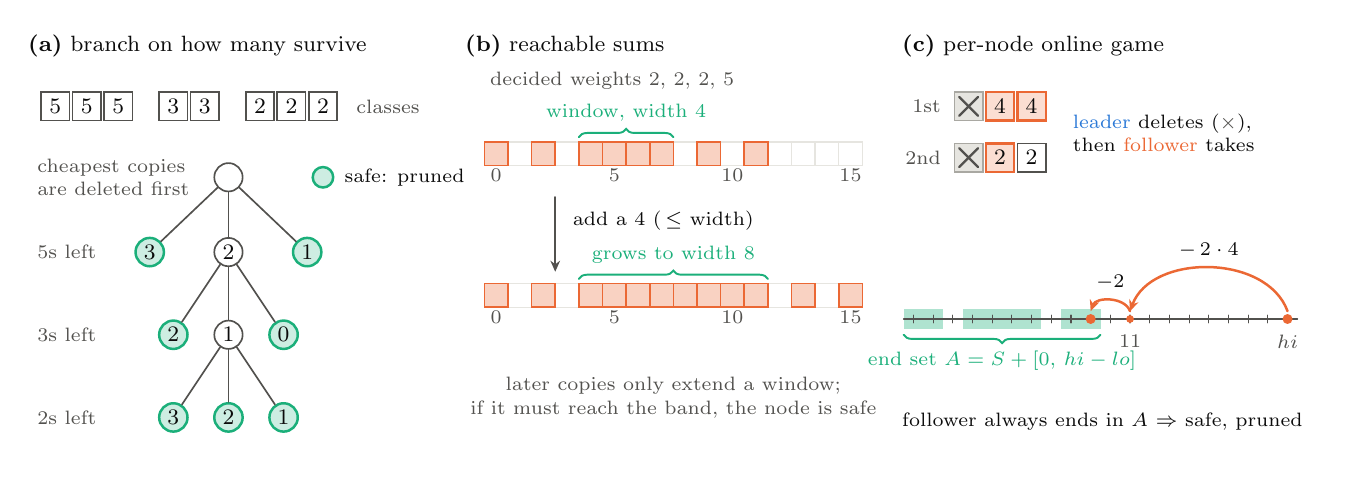
\begin{tikzpicture}
  % fixed page: 6.5 in x 2.2 in including the 2 pt border
  \useasboundingbox (0,0) rectangle (16.37,5.45);

  % =================== (a) search over survivor counts ===================
  \begin{scope}[shift={(0,0)}]
    \node[ptitle] at (0,5.22) {\textbf{(a)} branch on how many survive};
    % the classes: equal weights side by side
    \foreach \x in {0.35,0.75,1.15} \node[copy] at (\x,4.45) {5};
    \foreach \x in {1.85,2.25} \node[copy] at (\x,4.45) {3};
    \foreach \x in {2.95,3.35,3.75} \node[copy] at (\x,4.45) {2};
    \node[small, text=ink2, anchor=west] at (4.05,4.45) {classes};

    % the tree
    \node[open] (r) at (2.55,3.55) {};
    \node[safe] (a3) at (1.55,2.6) {3};
    \node[open] (a2) at (2.55,2.6) {2};
    \node[safe] (a1) at (3.55,2.6) {1};
    \node[safe] (b2) at (1.85,1.55) {2};
    \node[open] (b1) at (2.55,1.55) {1};
    \node[safe] (b0) at (3.25,1.55) {0};
    \node[safe] (c3) at (1.85,0.5) {3};
    \node[safe] (c2) at (2.55,0.5) {2};
    \node[safe] (c1) at (3.25,0.5) {1};
    \foreach \p/\c in {r/a3,r/a2,r/a1,a2/b2,a2/b1,a2/b0,b1/c3,b1/c2,b1/c1}
      \draw[tedge] (\p) -- (\c);
    \node[small, text=ink2, anchor=west, align=left] at (0.0,3.55)
      {cheapest copies\\ are deleted first};
    % level labels
    \node[small, text=ink2, anchor=west] at (0.0,2.6) {5s left};
    \node[small, text=ink2, anchor=west] at (0.0,1.55) {3s left};
    \node[small, text=ink2, anchor=west] at (0.0,0.5) {2s left};
    % key
    \node[safe, minimum size=0.26cm] at (3.75,3.55) {};
    \node[small, anchor=west] at (3.9,3.55) {safe: pruned};
  \end{scope}

  % =================== (b) a window of reachable sums ===================
  \begin{scope}[shift={(5.55,0)}]
    \node[ptitle] at (0,5.22) {\textbf{(b)} reachable sums};
    \def\c{0.3}  % cell size
    \def\x0{0.25}
    % strip 1: decided weights 2,2,2,5
    \node[small, text=ink2, anchor=west] at (\x0-0.05,4.78) {decided weights 2, 2, 2, 5};
    \foreach \t in {0,...,15}{
      \draw[grid, line width=0.5pt, fill=white] (\x0+\t*\c,3.7) rectangle ++(\c,\c);
    }
    \foreach \t in {0,2,4,5,6,7,9,11}{
      \draw[follower, line width=0.6pt, fill=follower!30] (\x0+\t*\c,3.7) rectangle ++(\c,\c);
    }
    \foreach \t in {0,5,10,15}
      \node[small, text=ink2, anchor=north, inner sep=1pt] at (\x0+\t*\c+\c/2,3.7) {\t};
    \draw[brace, cert] (\x0+4*\c,4.06) -- (\x0+8*\c,4.06)
      node[midway, above=2pt, text=cert, small] {window, width 4};

    % arrow: add a weight
    \draw[-{Stealth[length=4pt,width=3.5pt]}, ink2, line width=0.6pt]
      (\x0+0.9,3.3) -- (\x0+0.9,2.35);
    \node[small, anchor=west] at (\x0+1.0,3.0) {add a 4 (\,$\le$ width)};

    % strip 2: after one more copy of 4
    \foreach \t in {0,...,15}{
      \draw[grid, line width=0.5pt, fill=white] (\x0+\t*\c,1.9) rectangle ++(\c,\c);
    }
    \foreach \t in {0,2,4,5,6,7,8,9,10,11,13,15}{
      \draw[follower, line width=0.6pt, fill=follower!30] (\x0+\t*\c,1.9) rectangle ++(\c,\c);
    }
    \foreach \t in {0,5,10,15}
      \node[small, text=ink2, anchor=north, inner sep=1pt] at (\x0+\t*\c+\c/2,1.9) {\t};
    \draw[brace, cert] (\x0+4*\c,2.26) -- (\x0+12*\c,2.26)
      node[midway, above=2pt, text=cert, small] {grows to width 8};
    \node[small, text=ink2, align=center] at (\x0+2.4,0.75)
      {later copies only extend a window;\\ if it must reach the band, the node is safe};
  \end{scope}

  % =================== (c) the per-node online game ===================
  \begin{scope}[shift={(11.1,0)}]
    \node[ptitle] at (0,5.22) {\textbf{(c)} per-node online game};
    % class 4: leader deletes one copy, follower takes the other two
    \node[small, text=ink2, anchor=east] at (0.62,4.45) {1st};
    \gonecopy{(0.85,4.45)}{4}
    \node[taken] at (1.25,4.45) {4};
    \node[taken] at (1.65,4.45) {4};
    % class 2: leader deletes one copy, follower takes one of the two left
    \node[small, text=ink2, anchor=east] at (0.62,3.8) {2nd};
    \gonecopy{(0.85,3.8)}{2}
    \node[taken] at (1.25,3.8) {2};
    \node[copy]  at (1.65,3.8) {2};
    % key
    \node[small, anchor=west, align=left] at (2.05,4.12)
      {{\color{leader}leader} deletes ({\color{ink2}$\times$}),\\
       then {\color{follower}follower} takes};

    % number line of the follower's residual, 0 .. hi = 19
    \def\s{0.25}\def\x0{0.15}\def\y{1.75}
    % end set A = S + [0, hi - lo], S = {0,3,5,8}, hi - lo = 1
    \foreach \t in {0,1,3,4,5,6,8,9}
      \fill[cert!35] (\x0+\t*\s-\s/2,\y-0.13) rectangle ++(\s,0.26);
    \draw[ink2, line width=0.6pt] (\x0-\s/2,\y) -- (\x0+19.5*\s,\y);
    \foreach \t in {0,...,19} \draw[ink2, line width=0.4pt] (\x0+\t*\s,\y-0.05) -- ++(0,0.1);
    \draw[brace, cert, decoration={mirror}] (\x0-\s/2,\y-0.2) -- (\x0+9.5*\s,\y-0.2)
      node[midway, below=2pt, text=cert, small] {end set $A = S + [0,\, hi-lo]$};
    \node[small, text=ink2, anchor=north, inner sep=1pt] at (\x0+19*\s,\y-0.16) {$hi$};
    \node[small, text=ink2, anchor=north, inner sep=1pt] at (\x0+11*\s,\y-0.16) {11};
    % the follower's moves
    \draw[follower, line width=0.9pt, -{Stealth[length=4pt,width=3.5pt]}]
      (\x0+19*\s,\y+0.1) to[out=110, in=70] node[midway, above, small, text=ink] {$-\,2\cdot 4$}
      (\x0+11*\s,\y+0.1);
    \draw[follower, line width=0.9pt, -{Stealth[length=4pt,width=3.5pt]}]
      (\x0+11*\s,\y+0.1) to[out=110, in=70] node[midway, above, small, text=ink] {$-2$}
      (\x0+9*\s,\y+0.1);
    \fill[follower] (\x0+19*\s,\y) circle (1.8pt);
    \fill[follower] (\x0+11*\s,\y) circle (1.4pt);
    \fill[follower] (\x0+9*\s,\y) circle (1.8pt);
    \node[small, align=center] at (2.55,0.45)
      {follower always ends in $A$ $\Rightarrow$ safe, pruned};
  \end{scope}
\end{tikzpicture}
\end{document}
